\documentclass{ctexart}
\usepackage{bm, hyperref}

\begin{document}
\title{OSH项目调研报告}
\author{马凯,金孜达,刘时,徐亦尧,李文睿}
\maketitle
\tableofcontents
\section{项目背景}
物联网的原名是Internet of Things,即物物相联的互联网。在信息化大潮下,物联网的重要性将日趋突出。未来民用设备的智能化将主要通过物联网技术实现。

目前,物联网仍在早期快速发展阶段。物联网技术主要依托于现在的嵌入式设备,但增加了设备间互相联接、通讯的能力。为了降低物联网系统的总体成本,一般来说设备的性能不是特别强大,相当强调硬件与软件的配合:硬件强一分便是浪费、弱一分就无法实现功能。此外,物联网设备由于其应用的特点,也强调实时性,从而提供流畅的用户体验。因此,嵌入式物联网设备的开发门槛较高,需要程序员对硬件有足够深入的理解,这限制了物联网设备的开发、推广与应用。

其中,开发嵌入式物联网设备的一个重要门槛是数据高效的存储与传输。目前嵌入式设备通常使用闪存作为数据存储,但由于内存大小、CPU性能限制,无法使用功能强大的操作系统和文件系统,这导致开发者常常需要通过地址直接操作物理存储,严重限制了开发效率和系统的可扩展性。为此,我组提出了Internet-aware Real-time File System for IoT Systems with Limited Resources(面向资源有限的物联网系统的互联网感知实时文件系统)作为题目,以期降低物联网系统开发难度,并面向尽量多的应用场景,允许开发者进行进一步裁剪和二次开发。
\section{立项依据}
为此,我组进行了广泛调研。我组主要调研了嵌入式文件系统和分布式文件系统(详见调研部分)。其中,嵌入式文件系统主要特点是低资源消耗,但性能和功能有限制;分布式文件系统主要运行在服务器上,资源比较宽裕,性能较高,功能丰富。这两者看似矛盾,但若作出一定取舍,将完美契合于物联网应用。

基于这些调研,我们提出了Internet-aware Real-time File System for IoT Systems with Limited Resources(面向资源有限的物联网系统的互联网感知实时文件系统)作为题目。

我组题目的预期目标为:
\begin{enumerate}
	\item 资源占用低:内存消耗少,CPU占用少;
	\item 满足一定实时性要求;
	\item 可扩展性:可以快速适应不同物联网应用场景和快速变化的需求;
	\item 可伸缩性:当设备的存储(如闪存加倍时)将可被设备透明地利用;
	\item 适用于网络:透明化地将流数据在本地进行缓存。
\end{enumerate}
这些目标若实现,将大大降低物联网应用开发门槛。

在调研过程中,我们也进行了深入讨论。我们主要对物联网应用的需求进行了研究和讨论,在“资源占用”和“开发效率”方面达成共识。对于分布式文件系统,我们主要讨论了现有的成熟方案,找出了其中的优势和不足,为项目的具体设计提供灵感。
\section{前瞻性/可行性分析}
当该项目成功实现时,未来的嵌入式物联网设备开发一个难点将被去除。开发者将有望通过一个简单、易用、统一、可扩展的接口开发嵌入式设备,轻松地支持多种多样的设备。

在调研过程中,我们调研了现有的嵌入式文件系统和分布式文件系统,认为现有的嵌入式文件系统和分布式文件系统都不适用于物联网设备,理由如下:
\begin{enumerate}
	\item 嵌入式文件系统一般用于嵌入式操作系统。部分嵌入式文件系统过于强调接口兼容性,这使得一些更高性能、更低消耗的设计很难实现。
	\item 分布式文件系统除去资源消耗问题,还有抽象层次过高的问题,在嵌入式场景下没有任何用处。
\end{enumerate}
为此,我们提出以下改进想法:
\begin{enumerate}
	\item 放弃与传统文件系统的兼容性。对于嵌入式设备来说,这样的兼容性好处远不如坏处多
	\item 改进流数据的存储性能。一些传感器将源源不断地产生数据,这些数据的存储、处理和传输使用一般的文件系统并不容易做。
	\item 实现C/S模型的分布式文件系统,并且只传输流数据。服务端实时接收数据。客户端将尝试立即发送数据,如果网络情况较差,可以在本地进行缓存。
\end{enumerate}
基于现有的低消耗实时操作系统,这些目标对一门课程的大作业来说也是可行的。详细的设计与分析见可行性报告。
\section{周边项目调研}
\subsection{Coda 文件系统}
Coda文件系统是卡内基梅隆大学于1990年发布的文件系统,是对AFS2的改进。Coda最大的特色是支持离线操作,并能在上线后自动完成同步,这使得Coda非常适用于网络连接不稳定的使用场景。\cite{Coda}
\subsubsection{特点}
\begin{itemize}
	\item 离线操作
	\begin{itemize}
		\item 可从离线客户端上重新整合信息:使用客户修改日志
		\item 带宽适应性
	\end{itemize}
	\item 容错性
	\begin{itemize}
		\item 读/写副本服务器
		\item 服务器间的冲突解决
		\item 处理网络异常导致服务器被分隔的情况
		\item 处理客户端离线的情况
	\end{itemize}
	\item 性能和可伸缩性
	\begin{itemize}
		\item 客户端持有文件、目录、属性的持久性缓存
		\item 会写缓存
	\end{itemize}
	\item 安全性
	\begin{itemize}
		\item 类似Kerberos的身份认证
		\item 访问控制列表
	\end{itemize}
\end{itemize}
\subsubsection{架构与实现}
Coda采用C/S架构,挂载文件系统者为客户端,提供存储空间为服务端。
\subsubsection{客户端}
当Coda作为客户端运行时,只需挂载 /coda即可访问服务器上所有可访问的文件,且所有客户端看到的命名空间都是一样的。

当用户程序访问文件时,VFS请求本地缓存管理器,若不存在本地缓存,则向服务器发出请求获取该文件作为缓存。若无网络、服务器无应答,则进入离线模式。

一旦缓存命中,则所有操作均可在本地完成。文件被关闭时,客户端向服务器发送一个新文件;发生文件系统操作(创建文件夹、符号链接等)时,也向服务器通知。
\subsubsection{离线操作下的缓存一致性}
在线时,客户端将所有操作同步传递给服务器,但若客户端不在网络上或服务器不在线,则进入离线模式。该模式下有一些无法挽救的错误,如访问没有缓存的远程文件,只能向程序报告错误。

为支持离线操作,在操作超时时,缓存管理器将在客户端记录修改,作为客户端修改日志(CML)。当客户端和服务器重新建立连接时,服务器将重播日志来更新服务器上的文件。

Coda有时会故意放弃一致性而追求高性能

有些文件十分重要,我们希望能始终保持版本最新。Coda将经常向服务器请求这些文件的最新版本。

在重整合过程中,可能出现编辑冲突。Coda有时可以自动解决冲突,有时需要用户介入。
\subsubsection{卷、服务器和服务器副本}
在服务器上,Coda的文件并不使用传统文件系统存储,而是使用卷(代表一整个目录)。典型地,一个服务器上可能有上百个卷,每个卷平均约10MB。Coda将卷/目录信息、访问控制列表和文件属性信息存放在原始分区上。Coda使用基于日志的可恢复虚拟内存保证性能和一致性,在服务器崩溃时,能确保可以恢复到一个一致状态。

每个卷都有名字和ID,可以挂载在 /code下的任意位置。而对用户来说这一切都是透明的,用户只能看到一个目录。存在一个特殊卷,将在启动时自动挂载为 /coda根目录。

每个文件使用32位三元组Fid标识 (VolumeId, VnodeId, Uniquifier)。VolumeId标识文件所在的卷,VnodeId是文件的“inode”编号,Uniquifier用于避免冲突。Fid在一个Coda服务器的集群上是唯一的。

客户端访问服务器上的文件时,首先查找对应的VolumeId,请求的信息包括服务器列表和每个服务器上的本地卷ID。文件操作可以描述为read-one, write-many,同一文件在不同服务器上有多个副本,提高可靠性和可用性。

但由于种种因素,服务器之间一旦出现分区就有可能造成服务器之间的不一致。客户端在每次发送请求时会向所有服务器发送请求并比较服务器上文件的版本,如果服务器上的文件版本不一致,则客户端发起冲突解决,由服务器解决问题。
\subsubsection{工作贡献}
在Coda之前的网络文件系统对网络条件要求很高。在大型网络中,网络和机器出现异常情况的概率很高,为此应该支持离线操作。Coda通过客户修改日志、服务器重放、自动维修来解决了这个问题。
\subsubsection{不足之处}
Coda的实时性不高。在在线模式下,始终要求最新版本的文件也是轮询服务器来实现的,这将无法满足高性能、大流量的流式数据传输需求。

Coda作为1990年的文件系统,有很多设计已经无法满足现在的文件系统需求。如一个卷的平均大小仅约为10MB,这在现在看来是非常小的。
\subsection{星际文件系统}
\subsubsection{摘要}
星际文件系统(InterPlanetary File System,缩写IPFS,下用IPFS代替)是一个试图用相同的文件系统来连接所有计算机的端对端(P2P)分布文件系统。IPFS 与万维网的结构类似,但它也可以视作使用一个Git仓库交换数据的BitTorrent单群。 IPFS提供了一个高吞吐的区块存储模型,并带有基于内容寻址的超链接,从而形成一个广义的Merkle有向无环图。它由分布的散列表、带有激励机制的区块交换系统和自我认证的命名空间构成,没有单点故障,节点之间也不需要互相信任。
\subsubsection{IPFS 设计}
IPFS借鉴了以前端对端系统中的优秀想法,比如DHT,BitTorrent,Git和SFS等。在IPFS中,每份文件以及其中所有的区块都有一个唯一的指纹,被称作加密散列;IPFS对每个文件追踪历史版本并删除冗余的复制版本;每个网络节点无需存储全部数据,仅存储它感兴趣的一部分,以及一些索引信息来帮助它从其他机器上下拉数据;查询文件的时候,它通过网络来寻找含有此文件的节点;IPFS 使用星际命名空间(InterPlanetary NameSpace,缩写IPNS,下用IPNS代替)来将文件的散列映射为人类可读的名字。

IPFS 协议采用端对端模式,所有节点都是平等的。文件与数据结构统称IPFS对象。节点在本地存储IPFS对象并使用网络互相传递。 IPFS协议分为7个不同功能的子协议:
\begin{enumerate}
	\item 身份协议:管理节点身份生成与验证。
	\item 网络协议:使用各种已有的底层协议管理端对端连接。
	\item 路由协议:通过维护信息帮助定位特定的端或对象,同时对本地或者远程请求相应。
	\item 交换协议:使用新的区块交换协议(BitSwap)有效地分配区块,该协议类似于市场交易机制。
	\item 对象协议:使用Merkle有向无环图的结构,用链接来建立不可变动的对象,比如文件数据结构和交流系统等。
	\item 文件协议:一个类似Git的带版本管理的文件系统。
	\item 命名协议:一个自我认证的可变的命名空间。
\end{enumerate}
\paragraph{身份协议}
节点通过NodeID辨认身份,NodeID是通过S/Kademlia加密谜题来对公钥做散列得到的,公钥和私钥使用口令加密存储在各自的节点中。

在每次启动时,用户都可以选择实例化一个新的节点,不过这个操作会流失他们在网络上原先的累计收益,所以一般他们都愿意保留原先的节点。

在第一次连接时,双端交换公钥,并检查公钥的散列与NodeID是否一致,若不一致则拒绝连接。

IPFS 也接受使用多种散列函数,所以在交换公钥的时候也可以在头部加入自己的散列函数的代码。
\paragraph{网络协议}
通常,一个节点时常与数百个网络中的其他节点沟通信息,有时也可能会跨越整个网络。IPFS网络协议带有如下特性:
\begin{enumerate}
	\item 传输:IPFS可以使用任何传输协议,推荐使用WebRTC DataChannels或者uTP。
	\item 可靠性:如果下层的协议没有保证可靠性,那么IPFS也会提供可靠性。
	\item 连通性:使用ICE NAT遍历技术。
	\item 完整性:可选,使用散列校验和检查消息的完整性。
	\item 权威性:可选,使用发送者的公钥和HMAC算法确认消息的权威性。
\end{enumerate}
\paragraph{路由协议}
节点需要一套路由系统来帮助它们找到其他端的网络地址,以及那些可以提供特定对象的端。IPFS使用一个基于在S/Kademlia和Coral上的DSHT来达成此功能。IPFS DHT通过区块的大小区分它们的存储方法,例如小于等于1KB的区块DHT直接存储,大于1KB的区块DHT将存储引用信息(能提供此区块的对象的NodeID列表)。
\paragraph{交换协议}
IPFS使用BitSwap协议交换区块。类似于BitTorrent,BitSwap中的端有一条需求列表记录它想要的区块,也有一条提供列表记录它能提供区块。BitSwap的机制类似于一个永恒的市场,在这里节点可以自由地获取和提供任意存在的区块。一些区块可能来自于毫无关联的文件,不过节点也可以一起打包出售。

在BitTorrent里,为了防止有些节点只是抓取数据但从不提供,它使用了投桃报李的策略来惩罚这些节点。在BitSwap里也定义了类似的交换意愿。在端对端中,记债务比
\[
	r = \frac{bits\_I\_sent}{bits\_I\_receive+1}
\]并定义发送意愿
\[ P_{(message\_willing\_to\_send|r)} = 1 - \frac{1}{1+e^{6-3r}}
\]
在每次发送或者接收数据后,更新r。可知,如果对方接受的数据与发送的数据的比例上升,那么我方的发送意愿将降低。当这个比例在1附近的时候,发送意愿大约在0.95;若比例提升到2,其意愿将降低到0.5;若比例超过3.6,则意愿迅速降为0.01以下。该策略可以防止通过大量创建全新节点然后纯粹为了拉取数据的行为。

BitSwap协议要求每个节点各自保存自己的一份账本存储这些信用信息,也包括自己的。在双端建立连接时,它们需要交换账本并保持信息一致。如果不一致,也可建立新账本,但会损失过去的信誉或债务。为防止恶意节点故意丢失账本来欺骗节点,对方也可以认为丢失账本者不可信,从而直接拒绝交易。

对象协议

DHT和BitSwap为IPFS构成一个庞大的端对端系统,用于快速可靠地储存和分布区块。IPFS建立了一个Merkle有向无环图,其将对象用加密散列连接起来。这是一个广义的Git数据结构。Merkle有向无环图为IPFS提供了许多有用的特性,如:
\begin{itemize}
	\item 内容寻址:所有内容都用它的多个散列校验和唯一定位。
	\item 防篡改:所有的内容都可通过校验和检验,IPFS可以据此检测被篡改或损坏的数据。
	\item 去重:拥有一致内容的对象视作等价,也只存储一次。
\end{itemize}
IPFS用散列唯一确定路径,所以以下路径都是等价的:
/ipfs/<hash of a>/b/c
/ipfs/<hash of b>/c
/ipfs/<hash of c>
\paragraph{文件协议}
IPFS的文件结构与Git非常接近,故不做表述。
\paragraph{命名协议}
IPFS使用内容来给文件寻址,但是文件是变动的,需要找到一种方法使得IPFS能在相同的路径找到变动的数据。IPFS认为,对象是永恒存在的,从而其采用了类似Git的版本管理,其中对象是不变的,但是引用确是可变的。

在IPNS中,为每个节点建立如下命名空间:

/ipns/<NodeID>

其下的内容不按照内容寻址方式建立,而是使用子目录路由协议。
\subsubsection{IPFS实际使用案例}
土耳其官方不能封禁的维基百科

土耳其在2017年4月封禁了维基百科。一些黑客行为主义者制作了一份维基百科的副本,并使用IPFS的方式在线发布。因为IPFS搜索内容的方式是从最近可用的副本中选择一个下载,用一个IPFS地址理论能找到任何一个副本,所以官方封掉一部分副本后,还可以找到另一份副本解决问题。

加泰罗尼亚独立公投网站复刻

加泰罗尼亚在2017年10月1日举行公投,此前几天,西班牙法院判定公投官网违法并予以阻拦。加泰罗尼亚海盗党使用IPFS复刻公民投票网并成功举行公投,随后在同年10月27日宣布独立。
\subsubsection{优点与不足}
\paragraph{优点}
分布式的文件系统减少了存储需求,版本管理使得历史可追溯,同时也可以设置成允许有多个副本,使得其能够做到更强的容错性,弱化垄断力量的介入,保证民主自由的进行。
\paragraph{不足}
路由的算法实质上在大网络里效率并不是特别高,而市场化的区块交易机制也依然会出现所有市场经济该出现的典型问题,且保存所有版本实质也增加了存储开销,在没必要保存历史的情况下是没有意义的。
\subsection{百度文件系统(Baidu File System)}
\subsubsection{介绍}
百度文件系统(以下简称BFS)是一个为支持实时应用而设计的分布式文件系统。类似于其他分布式文件系统,BFS具有高容错性。但与此同时,BFS还兼具低读写延迟和高吞吐量的特性。\cite{BFS}
\subsubsection{特性}
\begin{enumerate}
	\item 持续可用性:Nameserver 多节点冗余,并使用Raft共识算法维护其一致性,单个节点宕机不影响整体可用性。
	\item 高吞吐:高性能的数据引擎能最大化IO的吞吐量。
	\item 低延时:全局负载均衡,自动检测并规避慢速节点。 //似乎尚未实现
	\item 可线性扩展:支持多数据中心的架设及1w+数据节点管理。
\end{enumerate}
\subsubsection{结构:共五层}
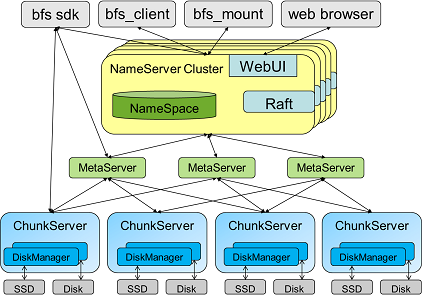
\includegraphics[width=\textwidth]{bfs.jpg}
由底至上:
\begin{enumerate}
	\item 硬件
	\item 单机节点ChunkServer:管理底层硬件
	\item MetaServer:为NameServer分担压力
	\item NameServer:类似于hdfs的namenode,但是一个集群而非单节点,这样可以解决部分可用性和性能瓶颈的问题。\footnote{hdfs中分Namenode和Datanode两种节点,是主从式结构。其中,Namenode负责管理文件系统的名字空间namespace以及客户端对文件的访问,而Datanode则负责节点存储。这种设计简化了系统的架构,因为存储数据无需经过Namenode。}
	\item 外层:用户接口/本地服务/sdk等
\end{enumerate}
\subsubsection{总体设计}
\begin{enumerate}
	\item 主备master结构:
	\begin{itemize}
		\item master之间通过一致性协议保持同步,每个master都存储所有信息。
		\item master的数据是落地(即被储存在持久化存储设备,如硬盘中)的,不一定非得全内存,通过LRU cache算法保证热点访问的快速响应。
	\end{itemize}
	\item 文件分块
	\begin{itemize}
		\item 文件是否分块决定了能否支持大文件
		\item 文件名信息是否存储在master决定了是否支持小文件
		\item 折衷是对大文件才分块,小文件(<100G)不分块;创建文件夹时指定可否list,可list的必须存在目录树中,不可list的可以哈希到chunkserver,让chunkserver去维护meta信息。
	\end{itemize}
	\item 文件meta信息(元数据:描述文件属性的数据)
	\begin{itemize}
		\item 文件meta信息存储在master会导致master负载过高(内存,cpu)。 我们选择对于不分块的文件,将文件meta存储在chunkserver,如果用户要list,那仅需要访问master,但如果要获取文件大小等信息,那就必须得访问对应的chunkserver了,master仅存储namespace和每个文件在哪些chunkserver上。
	\end{itemize}
	\item 写数据流
	有两个选择:
	\begin{itemize}
		\item client写一份,然后chunkserver通过复制链创建多副本,优势是client带宽占用低;
		\item client一次写多份,优势是可以多写一份,并在写的过程中抛弃慢节点。
	\end{itemize}
	\item 名称空间
	使用LevelDB存储:可以简单的将整个目录结构平展开,并提供高效的文件创建、删除、list和rename操作。例. 对于实际目录结构:

	/home/dirx/

	/filex

	diry/

	/filey

	/tmp/

	filez

	存储格式为:

	1home -> 2

	1tmp -> 3

	2dirx -> 4

	2diry -> 5

	3filez -> 6

	4filex -> 7

	5filey -> 8
\end{enumerate}
\subsubsection{Master(NameServer)高可用设计方案:}
\begin{enumerate}
	\item 背景:在BFS中,NameServer负责管理文件meta信息以及所有ChunkServer的状态信息,是整个系统中唯一拥有全局信息的模块,同时也成为了系统的单点。NameServer的不可用会直接导致文件系统的瘫痪,于是提高NameServer的可用性至关重要。
	\item 结构:将NameServer 扩展为集群,Client只与集群Leader进行交互。每一个NameServer中有一个同步模块(Sync),负责集群间的状态同步,保证元数据的一致性。
	\begin{itemize}
		\item Sync模块

		Sync模块主要有两个功能,选主和日志同步。选主操作就是在NameServer中确定唯一一个Leader,并且在Leader异常后迅速选出新任Leader。日志同步操作实际上就是同步NameServer中所有需要落地的数据写操作。Sync模块设计为与NameServer松耦合,仅暴露必须接口,内部可以采用任意一致性协议实现。这样的设计使得我们可以实现多种一致性方案,以满足不同程度的可用性及性能需求。当前我们采用Raft协议实现。
		\item Leader

		NameServer集群中的Leader负责接收和响应Client的请求,并把所做出的决定通过Sync通知集群中其他NameServer。Leader只在通知成功后才会向Client返回操作成功。
		\item Leader

		NameServer集群中的Leader负责接收和响应Client的请求,并把所做出的决定通过Sync通知集群中其他NameServer。Leader只在通知成功后才会向Client返回操作成功。
	\end{itemize}
	\item 主要流程操作方案:
	\begin{itemize}
		\item 对写操作(改变文件meta信息的操作,包括Create、Delete和Rename):

		同步结果的方案:Leader在收到操作后先对数据库打一个快照,检查完合法性后,在提交给Sync之前就将数据写入本地数据库。之后再将操作提交给Sync,Sync返回扩散成功后,Leader将快照删除并给向Client返回成功。在Sync返回成功前,所有的读请求都会读快照之前的数据,也就是说Client不会读到还未扩散成功的数据。

		同步操作的方案:Client向Leader Nameserver发起请求,Leader收到请求后,对所需操作的路径加锁,检查操作合法性。如果操作是合法的,Leader将需要落地的数据通过Sync扩散给从Nameserver。Sync模块返回扩散成功后,Leader向Client返回操作成功。从NameServer收到提交操作的指令后,无需检查操作合法性,直接根据指令执行操作更改状态机和内存结构。

		两种方案各自有一定的局限性:同步结果的问题在于当操作的结果很大(例如删除目录下所有文件),可能超出内存大小范围,从而很难保证操作原子性。同步操作基于一个假设:Leader和从NameServer将同一个指令应用到状态机及更改内存状态所产生的结果严格一致。

		对扩散的失败,例如RPC超时、写失败等需要重试处理,如果超过一定重试次数,则均视为Nameserver集群不可用,需人工介入处理。各一致性协议对于扩散失败的定义不同,例如Raft中,大于半数成员收到消息便认为扩散成功;主从模式中主或从任意一方写失败均认为是扩散失败。
		\item 对读操作:

		因为数据扩散存在延时,只有Leader掌握最新的数据,所以只有Leader可以响应Client的读请求。Client向Nameserver集群中任一实例发起读请求,如果正好是Leader接收到了请求,则直接返回给Client结果;否则,从Nameserver返回读失败并告知当前Leader地址,Client向新Leader请求。
		\item 关于模式切换:

		主从方案有两种模式:主从模式和单主模式。严格的主从模式,需要日志成功同步给从后再向用户返回成功。这种情况一旦从宕机,会导致集群不可用。所以引入了单主模式,在从故障的情况下,依然可以提供服务。单主模式下,主将日志持久化到本地log,之后直接向用户返回结果。
		\item 关于主从切换:

		当主宕机时,需要将从切换为主。这时向从发送切换命令,从将自己的term加一,然后切换为主对外提供服务。term的作用主要为了标识曾经发生过主从切换,因为当前实现中,主的状态机中可能存在脏数据,之前的主作为从重启,而又没有清理自己的状态机,脏数据将不会被发现。在term机制下,之前的主以从的身份重启后,会发现有比自己term更高的主存在,会将自己的状态机和本地日志清理干净,然后等待主发送镜像。
	\end{itemize}
\end{enumerate}
\subsubsection{启发}
BFS的特殊之处有两点,其一是将系统分为NameServer和ChunkServer两个部分:众多ChunkServer各负责一块盘上文件的存储,而NameServer负责与Client通信控制存储。NameServer是整个系统的中心,但由于无需存储所有的文件内容,结构相较于传统的中心化存储系统有所简化。如果我们要做物联网设备的文件系统,可以考虑加入这样一个控制中枢,所有的系统控制操作全部在中心节点完成,而其他物联网设备全部视为存储节点,只需负责发送和接收文件内容信息,可能可以实现减轻物联网设备工作压力的目的。第二个特点是将NameServer集群化,提高了系统的可靠性。在规模不太大的系统中,为中心节点添加一个从节点作为备份就可能有效提高系统的可靠性,在我们的设计中也可以考虑这一点。
\subsection{Gnutella 项目}
\subsubsection{关于 Gnutella 项目}
Gnutella是一个用于分布式搜索和数字资源共享的协议,他的特色是它的点对点、非中心的模型。

在这个模型中,任何一个客户端同时也是一个服务器,反之亦然。所以Gnutella中给它们起了一个专门的名字叫做servent (是从“SERVer”和“cliENT”各取一部分组成的)。Servent提供客户端接口,用户通过这个接口可以提交查询并查看查询结果,同时,它们也可以接受查询请求,在本地数据中检索,并返回符合条件的结果。因为这种分布式属性,实现Gnutella协议的由servent组成的网络具有高度的容错性,一部分servent掉线并不会中断正在进行的网络操作。
\subsubsection{Gnutella协议}
\begin{enumerate}
	\item 连接Gnutella网络(Bootstrapping过程)

	为了连接Gnutella网络,servent需要发现并存储多个主机的地址,有四种方式
	\begin{enumerate}
		\item 调用一个GWebCache。这是一个有人上传到他们的Web服务器的PHP脚本。运行在用户计算机上的Gnutella程序调用脚本来获取计算机的IP地址,并获取最近完成相同事情的程序的IP地址。这让Gnutella程序能够找到彼此。
		\item 在握手期间,Gnutella程序在X-Try和X-Try-Ultrapeers头文件中告诉对方更多的IP地址。
		\item 有些地址以相同的方式洒在Pong message(reply to ping(discover hosts on network))中。
		\item Query hit(reply to query)也包含IP地址。
	\end{enumerate}
	\item 启动算法

	一般情况下,在一个会话期内,不要向web cache发送太多的请求,查询GWebCache的次数不应该超过一次。也就是说,一个用户掉线的时候,代替的方案是用本地主机的cache来存储发现的主机地址,并和GWebCache一起使用。
	\begin{itemize}
		\item 启动客户端并调入本地主机cache
		\item 使用本地主机cache连接GNet.
		\item 如果在X秒后还没有连接到GNet,查询一个随机的GWebCache.
		\item 等待最少Y秒后,向另一个GWebCache发送请求。(在第一次选取的GWebCache死机或者反应非常慢的情况下)
		\item 在Y秒后,如果第一次GWC调用还没有返回结果,每隔Z秒调用一个新的GWC,直到收到其中一个的响应。
		\item 一旦至少收到一个GWC的返回结果,只有在本地主机cache为空的情况下,           servent才应该在接下来的session中发送新的请求 (如果软件提供初始的主机cache,并且没有清除主机cache的选项,这种情况就不应该发生).
	\end{itemize}
	假设X,Y和Z的值分别为5秒、10秒和2秒,这样应该能够确保servent能够很快连接到GNet并把查询GWebCache的次数控制到最低。

	启动过程还应该确保servent不用经常连接一个远程主机,每秒钟少于一次是一个合理的界限。为了达到这个要求,一个解决办法就是确保本地主机cache中总是有足够多的主机,这样就能保证任何一个主机都不会在一分钟之内被再次试图连接。

	每一个servent在握手时都应该发送一个X-Try头,这个头给出这个servent可以尝试连接的主机列表,允许它在不用调用GWebCache的情况下得到新的主机地址。例如:

	X-Try:  1.2.3.4:1234, 1.2.3.5:6346, 1.2.3.6:6347

	servent应该发送适当数量的主机,一般在10到20之间。这些随着X-Try头发送的主机信息应该是确切的。所以,servent应该只选择那些最近(在发送X-Try头之前几分钟内)所知还在运行的主机。如果最近发现还在运行的主机数量少于10个,那发送时就少发送一些。如果servent实现了响应cache(参见3.4节),在响应信息中发现的主机可以认为具有空闲的时隙。但这不适用于在监控QueryHits中得到的主机信息。这样,在返回信息中得到的主机信息可以替换X-Try头中主机的位置,而QueryHits中发现的主机却不行。
\end{enumerate}
\subsubsection{握手协议}
一个Gnutella servent通过与当前在网络上的另一个servent建立连接的方式把自己连接到Gnutella网络。一旦第一个连接建立起来,网络可以提供更多的当前连接在网上上的主机地址。在得到当前在网上的另一个servent的地址时,首先建立一个到servent的TCP/IP连接,然后开始一个握手的消息序列。客户端是发起连接的主机,服务器是接受连接的主机。

(以下步骤来自于网络)
\begin{enumerate}
	\item 客户端建立一个到服务器的TCP连接
	\item 客户端发送“GNUTELLA CONNECT/0.6<cr><lf>”
	\item 客户端发送带有所有域的头,除了供应商自定义的特殊域,每个域以"<cr><lf>"结束,在整个头的最后添加一个额外的"<cr><lf>"
	\item 服务器以"GNUTELLA/0.6 200 <string><cr><lf>"应答,这里<string>应该是"ok",但是servent应该只查找"200"这个代码作为状态标志。
	\item 服务器发送自己信息头的全部,按照3规定的格式
	\item 如果客户端在解析完服务器发送的信息头以后,还希望继续,就发送"GNUTELLA/0.6 200 OK <cr><lf>"给服务器作为应答,就像4一样。否则,它需要返回一个错误码,并关闭这个连接。
	\item 客户端发送供应商自定义的信息头,与3的格式一样。
	\item 客户端和服务器按照3和5中得到的信息,按照自己的要求发送和接收二进制消息。

	例如:
	First-Field: this is the value of the first field<cr><lf>
	Second-Field: this is the value<cr><lf>
	of the<cr><lf>
	second field<cr><lf>
	<cr><lf>

	下面是一个客户端和服务器交互的例子。从客户端发送到服务器的数据列在左边,从服务器发送到客户端的数据列在右边。

	\begin{tabular}{cc}
		\hline
		Client                          &Server\\\hline
		GNUTELLA CONNECT/0.6<cr><lf>& \\
		User-Agent: BearShare/1.0<cr><lf>& \\
		Pong-Caching: 0.1<cr><lf>& \\
		GGEP: 0.5<cr><lf>& \\
		<cr><lf>& \\
		&GNUTELLA/0.6 200 OK<cr><lf> \\
		&User-Agent: BearShare/1.0<cr><lf> \\
		&Pong-Caching: 0.1<cr><lf> \\
		&GGEP: 0.5<cr><lf> \\
		&Private-Data: 5ef89a<cr><lf> \\
		&<cr><lf> \\
		GNUTELLA/0.6 200 OK<cr><lf>& \\
		Private-Data: a04fce<cr><lf>& \\
		<cr><lf>& \\
		{[binary messages]}&{[binary messages]} \\ 
	\end{tabular}
\end{enumerate}
\subsubsection{这个系统与我们所做系统的一些联系}
这个系统有一个好处就是,一个server就是一个client,也就是servent,这就使得各个节点之间的联系加强了。我们之前讨论过节点掉线后的同步问题情景,如果用这个servent解决的话,当一个节点掉线,其他节点进行更新后,这个节点再次上线,这时候的身份是client,其他距离这个节点近或者是符合其他某种规律的节点就可以及时的对掉线节点进行更新和同步。

我还想到的一点就是,我们要做一个类似于去中心化节点的系统,这个Gnutella协议也大致符合,每个节点既是服务器(数据更新的提供方)又是用户(数据更新的接收方),同时Gnutella协议方案也比较成熟,启动算法什么的都有,我们可以考虑在它上面加一点东西,难度适中。
\subsection{Google FS}
\subsubsection{GFS}
Google(gfs)是一个可扩展的分布式文件系统,用于大型分布数据密集型应用程序,在提供容错的同时运行在廉价的商品型硬件上,并为大量用户提供高集成性能。\cite{GFS}
\subsubsection{概况}
GFS是为Google日益增加的数据处理需求设计的,GFS与以前的分布式文件系统有着如性能,可扩展性,可靠性,可用性等很多共同的目标,但其设计由Google的应用工作负载和当前和预期的技术环境的关键观察所驱动,反映了一些早期的显着偏离文件系统设计假设,因此研究团队重新审视了传统选择并探索了根本上不同的观点。
\begin{itemize}
	\item 首先,组件故障是规范而非概念,由于数量庞大,某些组件会发生故障。持续监视,错误检测,容错和自动恢复必须要保证。
	\item 其次,系统上存储的文件大多都很大,定期处理大量TB级的文件时管理几十亿KB大小的文件是不切实际的,因此设计假设和参数要重新考虑。
	\item 第三,大多数文件都是以附加而不是覆盖的形式被修改,文件内的随机写入实际不存在,一旦被写入则只能被顺序读取,鉴于这种大型文件的访问模式,追加成为性能优化和原子性保证的重点,而在客户端缓存数据块则失去了吸引力。
	\item 第四,通过增加灵活性,共同设计应用程序和文件系统API可以使整个系统受益,如放宽了GFS的一致性模型,大大简化了文件系统,而不会给应用程序造成沉重的负担。还引入了一个原子追加操作,以便多个客户端可以并发地追加到一个文件中,而无需在它们之间进行额外的同步。
\end{itemize}
\subsubsection{设计综述}
\paragraph{设想}
\begin{itemize}
	\item 要定期监视检测故障,以及容错性和故障恢复
	\item 系统主要存储大文件,小文件也要支持,但不对其进行优化
	\item 两种文件读取方式:大型流阅读和小型的随机阅读
	\item 系统必须有有效的对同一文件进行并发附加的处理机制
	\item 高持续带宽比低时延更为重要
\end{itemize}
\subsubsection{Interface}
支持一般的创建、删除、打开、关闭、读写文件的功能。

GFS还支持快照和记录追加,记录追加可以让多个客户端同时向同一个文件追加数据而无需加锁。
\subsubsection{Architecture}
GFS由master和chunkservers组成,也可以轻易的在同一台机器上运行chunkserver和client。

文件被分为等大的块,每一块被64位的chunk handle(master根据块创建的时间产生)确定。每一块都在多个chunkserver上有备份,这样能确保稳定性,默认三份,用户可以指定备份级别。

master存储所有的元数据,如命名空间,访问控制信息,文件与chunk的对应关系,chunk的位置等,也控制系统级别的活动如垃圾清理,孤儿chunk的处理,chunk的合并等。master定期与chunkserver联系以传递指令和收集chunkserver的状态。

client则通过与master和chunkserver的沟通处理数据,将元数据处理交给master,而数据承载则直接交给chunkserver。

不论是client还是chunkserver都不缓存数据,因为这没有好处。
\subsubsection{single master}
用户添加文件时,直接将文件名及offset等信息发送给master,master添加文件信息并给client传回location及index,client再用此信息将文件传给chunkserver。
\subsubsection{chunk size}
chunk大小指定为64MB

好处:
\begin{itemize}
	\item 减少了client与master的沟通
	\item client可以在给定的chunk上进行更多操作,减少建立TCP连接需要的时间。
	\item 减少了master上元数据的大小。
\end{itemize}

缺点:hotspot
\subsubsection{metadata}
master上的metadata有namespace,文件与chunk的对应关系,chunk的位置。使用log使得系统升级更简单稳定。

master负责周期性的扫描,包括垃圾处理,错误恢复,为平衡负载的chunk合并等。

master不维护特定chunk的位置记录,只是在开始的时候与chunkserver通信,这解决了chunkserver的加入,离开,故障等时master与其的同步。

operation log包括元数据改变的历史记录,这非常重要,因此在远程的部分机器上也进行备份,master通过replay operation log来恢复文件系统状态。当log的size达到一定程度时,master检查状态,这样恢复的时候只要恢复最新的log上几条记录即可。checkpoint在能直接被map入内存的一个紧凑的B+树内,在启动时系统可以将log记录进新的log文件中,这样就不用delay启动期间的修改。checkpoint期间的fail不影响准确性,因为恢复操作会跳过未完成的checkpoint。
\subsubsection{Consistency Model}
GFS的一致性:
\begin{itemize}
	\item defined: 状态已定义,从客户端角度来看,客户端完全了解已写入集群的数据,例如,客户端串行写入且成功,此时的状态是defined
	\item consistent: 客户端来看chunk多副本的数据完全一致,但不一定defined,一般发生在多客户端并发更新时
	\item unconsistent: 多副本数据不一致
	\item undefined: 数据未定义
\end{itemize}
从修改过程看:
\begin{itemize}
	\item 串行over-write: over-write由客户端指定文件更新offset。当客户端是串行更新时,客户端自己知道写入文件范围以及写入数据内容,且本次写入在数据服务器的多副本上均执行成功。因此,本次写结果对于客户端来说就是明确的,且多副本上数据一致,故而结果是defined
	\item 并行Over-Write: 并行写入时多个客户端由于写入范围可能交叉而形成交织写。这时候,由于单个客户端无法决定写入顺序(只有主副本才能决定谁先写谁后写),因此,即使写入成功,客户端仍无法确定在并发写入时交叉部分最终写入结果,但是因为写入成功,所以多副本数据必然一致,即为consistent but undefined
	\item append: 客户端append操作无需指定offset,由chunk主副本根据当前文件大小决定写入offset,在写入成功后将该offset返回给客户端。因此,客户端能够根据offset确切知道写入结果,无论是串行写入还是并发写入,其行为是defined
	\item 在一系列的成功修改后,mutated file region被定义并且包含最后一次修改后的版本。之后按文件中的chunk顺序修改,并检测是否有过期的chunk,旧的chunk不会在与client通信时使用。
	\item 客户端缓存chunk的位置可能过期,于是client对缓存有时间限制,这会清除所有缓存信息。
	\item 组件的failure可能会损坏文件,因此GFS定期与chunkserver握手并使用checksum检查文件完整性,一旦出现问题,数据会迅速由其余可用的备份中恢复。除非在能够联系之前所有备份全部丢失,否则文件不可能彻底损坏(这种情况用户会收到error而不是损坏的文件)。
	\item 检查点允许编写者以增量方式重新启动,并无法成功处理在应用程序看来不完整的数据。
\end{itemize}
\subsubsection{租约(Lease)}
租约(Lease)是由GFS中心节点Master分配给chunk的某个副本的锁。持有租约的副本方可处理客户端的更新请求,客户端更新数据前会从Master获取该chunk持有租约的副本并向该副本发送更新请求。

租约本质上是一种有时间限制的锁:租约的持有者(chunk的某个副本)需要定期向Master申请续约。如果超过租约的期限,那么该租约会被强制收回并重新分配给其他副本。
\subsubsection{优点与不足}
\paragraph{优点}
负载均衡,容错性好,可扩展性强,满足POSIX语义,应用程序无需任何修改可直接使用GFS。
\paragraph{缺点}
Master启动时将所有元数据加载至内存中,由于gfs应用场景主要是大文件,对其影响并不严重,但限制了文件系统的可扩展性。
\subsection{物联网}
物联网(IoT)是物理设备,车辆,家用电器和嵌入有电子,软件,传感器,执行器和连接的其他物品的网络,这些物品能够连接和交换数据。每件事物都可以通过其嵌入式计算系统唯一识别,但能够在现有的互联网基础设施内进行互操作。\cite{IoT}

物联网允许物体被远程控制或感知,更便于将物理世界整合到计算机世界,减少了人为干预且提高了效率。设备依现有技术进行有效信息的收集,并通过物联网发送给其他设备。

这些系统可以负责收集从自然生态系统到建筑物和工厂等各种环境中的信息[41],从而在环境感知和城市规划领域找到应用,如在购物中寻找用户的购物习惯然后在他们喜欢的商品有折扣时进行提醒,还有智能家居,能源管理等。
\subsubsection{Architecture}
\begin{itemize}
	\item 物联网将是一个时间驱动架构
	\item 物联网也是一个语义网络,事件的意义基于本身的上下文
	\item 物联网之上是物联网应用层的体系结构,将物联网设备中的数据融合到web应用程序中以创建新的应用场景。
	\item 网络架构
	\begin{itemize}
		\item 随着大量设备加入物联网,IPv6将在处理网络层可扩展性方面发挥巨大的作用。
		\item 雾计算是防止极大量数据流过互联网的可行方案,边缘设备的计算能力可用于分析和处理数据,从而提供简单地实时可扩展性。
	\end{itemize}
\end{itemize}
\begin{thebibliography}{3}
	\bibitem{Coda}
	Coda:\url{http://www.coda.cs.cmu.edu/ljpaper/lj.html}
	\bibitem{BFS}
	BFS:\url{https://github.com/baidu/bfs}
	\bibitem{HDFS}
	HDFS:\url{hadoop.apache.org/}
	\bibitem{baidu}
	从百度文件系统看大型分布式系统设计中的定式与创新:

	\url{http://www.infoq.com/cn/presentations/form-and-innovation-in-large-distributed-system-design-from-baidu-file-system}
	\bibitem{GFS}
	Sanjay Ghemawat, Howard Gobioff, and Shun-Tak Leung: \textit{The Google File System}, \url{https://static.googleusercontent.com/media/research.google.com/en//archive/gfs-sosp2003.pdf}, Google, Oct 19-22, 2003
	\bibitem{IoT}
	\url{https://en.wikipedia.org/wiki/Internet_of_things}
\end{thebibliography}
\end{document}
